\chapter{Zaimplementowany system wspomagający autonomiczne lądowanie drona}
\label{cha:opis_implementacji}

%TODO Opis platformy sprzętowej + PCAM do osobnego rodziału + poszerzyć
\section{Zastosowana platforma sprzętowa}
\label{sec:zastosowana_platforma_sprzetowa}

W~pracy wykorzystano platformę Digilent~Zybo~Z7-20 z układem Zynq SoC (ang. \textit{System on Chip}) XC7Z020-1CLG400C oraz~kamerę~Digilent PCAM~5C. %TODO uzupełnić
Przeprowadzenie syntezy i~implementacji możliwe było przy użyciu darmowego oprogramowania Vivado oraz SDK w wersji WebPack -- używano wersji~2018.2. 
Układ dostępny na karcie określa się jako heterogeniczny tj. stanowi połączenie części rekonfigurowalnej (PL -- ang. \textit{programmable logic}) oraz systemy procesorowego z~dwurdzeniowym procesorem ARM Cortex-A9 taktowanym z~częstotliwością 667~MHz (PS -- ang. \textit{processing system}). 

%TODO W tym mejscu rozbudowa tj. omówinie architektury Zynq na podstawie schematu (są takie ładne obrazki dostępne) i kilka słów o komponentach.

%TODO potem to zdanie, nieco przeredagowane.
Do dyspozycji projektanta pozostawało 53 200 tablic LUT (ang. \textit{Look-up Table}), 106 400 przerzutników \textit{flip-flop} oraz 630 KB pamięci blokowej RAM. \\


%TODO Coś o kamerze, ale parametry. Te szczegóły techniczne to przy implementacji

Producent na swojej stronie internetowej zapewnia projekt demonstracyjny połączenia kamery i~płytki~\cite{projektPCAM}. Przez port szeregowy możliwa jest zmiana rozdzielczości, szybkości akwizycji ramek, współczynnika korekcji gamma, ustawień balansu bieli. Możliwe są następujące opcje dotyczące dwóch pierwszych parametrów:
\begin{itemize}
	\item 1280 x 720, 60 fps,
	\item 1920 x 1080, 15 fps,
	\item 1920 x 1080, 30 fps.
\end{itemize}
Testy pokazały również, że dla rozdzielczości 1280 x 720 większy jest kąt widzenia kamery. Kwestię tę opisano w~sekcji \ref{sec:wyznaczenie_kata_widzenia_kamery przy_roznych_ustawieniach}. Ze~względu na~powyższy fakt oraz przyspieszenie obliczeń, zdecydowano się na~najmniejszą dostępną rozdzielczość.\\
Pobrany projekt stanowił bazę do dalszych prac. 


%TODO Tu będzie początek tego nowego rozdziału. Przed modelem programowy proszę kilka zdań wstępu (co bedzie w treści)

\section{Implementacja i ewaluacja modelu programowego}
\label{sec:implementacja_modelu_programowego}

Model programowy został napisany w pakiecie Matlab przy wykorzystaniu funkcji dostępnych w~bibliotece \textit{Image Processing Toolbox}. 
Pozwoliło to na szybkie prototypownie systemu wizyjnego.
%TODO Przedstawić ogólny schemat algorytmu oraz go skórtowo omówić.

%TODO jest niejasne...bo jest mieszanie HW i modelu. Może proszę napisać dwa zdania o sekwencjach, bo chyba Pan zaczął od zwykłych, a potem z PCAM. Natomiast sprawę PCAM proszę "załatwić" w ten sposób, że ten opis ponież w części SW (jakiś subsectio), a tu się powołać

%TODO W kolejnych podrozdziałch uzasadnienie wyboru poszczególnych komponentów. Treść z "testy".
%TODO Znacznik. Potem przestrzenie barw i reszta


\subsection{} 


Aby możliwe było wprowadzanie ramek obrazu do modelu, należało umożliwić akwizycję obrazów na kartę SD. 
Uaktywniono interfejs procesora SD0, do~projektu w~SDK dodano bibliotekę ,,xilffs'' i,~korzystając z~funkcji systemu plików opisanych w~\cite{xilffs}, napisano zapis ramek do~pliku. 
Ze~względu na~prostotę pliku, składającego się jedynie z~nagłówka oraz wartości kolejnych składowych RGB, zdecydowano się na format ppm.\\
%TODO Ten opis powyżej trzeba nieco rozwinąć.

W~późniejszym stadium projektu, z~powodu różnic na obrazie zapisywanym na ramkę i~wyświetlanym na ekranie, zdecydowano się na zmianę tej koncepcji.  %TODO chyba na kartę.
%TODO a co to za róznice.
Zaimplementowano cały tor wizyjny w~części PL układu Zybo Z7-20 i~przechwytywano przetworzone obrazy wyświetlane na~monitorze. 
Dzięki takiemu podejściu podczas testowania widziano rzeczywiste wyniki przetwarzania.







\section{Implementacja sprzętowo-programowa}
\label{sec:implementacja_sprzetowo_programowa}
%TODO Krótki wstęp np. ogólny scheamt implementacji ze wskazaniem na podział HW/SW, taki schemat sprzętu (z peryferiami). Potem będzie Pan omawiał poszczególne komponenty. 

\subsection{Konwersja z przestrzeni barw RGB do YCbCr}
\label{subsec:konwersja}

Piksel w~przestrzenie barw YCbCr opisują trzy składowe: Y (luminancja), Cb (chrominancja, która wyraża różnicę między luminancją, a~kolorem niebieskim) oraz Cr ( chrominancja, która wyraża różnicę między luminancją,~a~kolorem czerwonym). 
Zaletą stosowania tej przestrzeni barw jest oddzielenie sygnału luminancji od~sygnałów chrominancji, pozwalające na~dokonywanie przetwarzania sygnału przy mniejszej zależności od~oświetlenia.
Konwersję z przestrzeni barw RGB do YCbCr wykonano zgodnie ze wzorem \ref{eq:ycbcr}. 
Przy implementacji wykorzystano sprzętowe mnożarki oraz sumatory.
\begin{equation}
\label{eq:ycbcr}
\begin{bmatrix} Y \\ 
				Cb\\
				Cr
\end{bmatrix}=
\begin{bmatrix} 0,299 & 0,587 & 0,114\\ 
				-0,168736 & -0,331264 & 0,5\\
				0,5 & -0,418688 & 0,081312
\end{bmatrix}
\begin{bmatrix} R\\
				G\\
				B
\end{bmatrix}+
\begin{bmatrix} 0\\
				128\\
				128
\end{bmatrix}
\end{equation}

%TODO Może schemat ?


\subsection{Binaryzacja}
\label{subsec:Binaryzacja}
% dobieranie progu: 2 multiplekser sterowany buttonem?
Piksel wyjściowy otrzymywał wartość maksymalną (kolor biały), jeśli wartości Cb i~Cr mieściły się pomiędzy wyznaczonymi eksperymentalnie progami. 
W~innym przypadku pikselowi przypisywana była wartość 0 (kolor czarny). 
Moduł binaryzacji pracował z zerową latencją.

%TODO Prawda jest taka, że to najlepiej zrobić z wykorzystaniem rejestrów AXI - to jest to przerobienia w kolejnej iteracji.


\subsection{Mediana}
\label{subsec:Mediana}
% obrazek wyznaczania kontekstu
% obrazek drzewa sumacyjnego

Mediana to operacja kontekstowa, w~której pikselowi wyjściowemu przypisuje się wartość środkową uporządkowanego zbioru wartości pikseli z~otoczenia piksela wejściowego. 
W~przypadku działania na~obrazie binarnym operacja taka może być przeprowadzona przez obliczenie sumy wartości pikseli wewnątrz kontekstu, a~następnie porównanie jej z~połową maksymalnej wartości tej sumy. 
Ze względu na łatwość implementacji oraz zadowalające wyniki filtracji, zdecydowano się na~rozpatrywanie kontekstu w~kształcie kwadratu o~boku 5~pikseli. 
Spowodowało to~konieczność zapamiętywania kontekstu piksela w~25 rejestrach oraz 4~linii obrazu w długich liniach opóźniających zbudowanych w~oparciu o~pamięć BRAM.
Schemat wyznaczania kontekstu przedstawiono na rysunku \ref{fig:kontekst}. 
Sygnały synchronizacji zostały doklejone do wartości piksela i~w~przedstawionej strukturze przesuwają się razem z~nim. 
Sumę wyliczano w~2~etapach, dodając najpierw elementy w~wierszach, potem sumując wyniki. 
Latencja modułu wynosiła 2, należało zatem opóźnić sygnały synchronizacji o~tyle taktów zegara. %TODO Modułu to więcej bo 4 linie i trochę.
\begin{figure}[h]
	\centering
	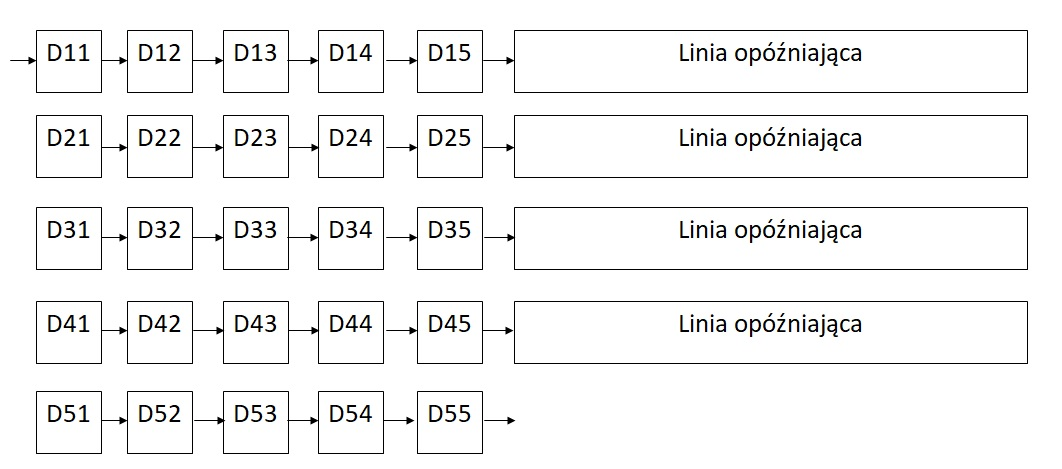
\includegraphics[width=\textwidth]{kontekst.jpg}
	\caption{Schemat wyznaczania kontekstu dla mediany, erozji i dylatacji.}
	\label{fig:kontekst}
\end{figure}  


\subsection{Erozja i dylatacja}
\label{subsec:erozja}

Erozja i dylatacja to~operacje morfologiczne, w~których pikselowi wyjściowemu przypisuje się wartość odpowiednio najmniejszego i~największego piksela w~sąsiedztwie piksela wejściowego. 
Sąsiedztwo piksela określa kształt i~rozmiar elementu strukturalnego. 
Podobnie jak w~przypadku mediany, zdecydowano się na~kwadrat o~boku 5~pikseli. 
Moduł erozji ustawia wartość piksela wyjściowego na~maksymalną wartość, gdy~w~sąsiedztwie znajdują się same białe piksele. 
W~module dylatacji zwracana jest wartość maksymalna, gdy przynajmniej jeden piksel w~sąsiedztwie ma kolor biały. 
Latencja modułów wynosi~1. %TODO Jw. skoro kontkst to 4 linie i trochę...

\subsection{Środek ciężkości i prostokąt otaczający}
\label{subsec:srodek_ciezosci}

Do wyznaczania środka ciężkości pikseli należących do~obiektu wykorzystano wzory \eqref{eq:m00}, \eqref{eq:m10} i~\eqref{eq:m01}.

\begin{equation}
\label{eq:m00}
m_{00}=\sum_{i=0}^{N-1}\sum_{j=0}^{M-1} x_{ij}
\end{equation}
\begin{equation}
\label{eq:m10}
m_{10}=\sum_{i=0}^{N-1}\sum_{j=0}^{M-1} i*x_{ij}
\end{equation}
\begin{equation}
\label{eq:m01}
m_{01}=\sum_{i=0}^{N-1}\sum_{j=0}^{M-1} j*x_{ij}
\end{equation}
gdzie:
\begin{eqwhere}[2cm]
	\item[$N$] szerokość obrazu w pikselach,
	\item[$M$] wysokość obrazu w pikselach,
	\item[$x_{ij}$] wartość piksela o~współrzędnych $i$, $j$ obrazu zbinaryzowanego.
\end{eqwhere}
Na ich podstawie obliczono środek ciężkości przy zastosowaniu wzorów \eqref{eq:xsc} i~\eqref{eq:ysc}.
\begin{equation}
\label{eq:xsc}
X_{sc}=\frac{m_{10}}{m_{00}}
\end{equation}
\begin{equation}
\label{eq:ysc}
Y_{sc}=\frac{m_{01}}{m_{00}}
\end{equation}
\begin{eqwhere}[2cm]
	\item[$X_{sc}$] współrzędna pozioma środka ciężkości,
	\item[$Y_{sc}$] współrzędna pionowa środka ciężkości.
\end{eqwhere}

W~module na podstawie sygnałów synchronizacji oraz wymiarów obrazka wyznaczono współrzędne aktualnie przetwarzanego piksela. 
Jeśli jest to piksel należący do obiektu, następuje zwiększenie wartości odpowiednich rejestrów zgodnie ze wzorami
\ref{eq:m00}, \ref{eq:m10} i~\ref{eq:m01}. 
Po przejściu przez całą ramkę obrazu wykonywane jest dzielenie na podstawie wzorów \ref{eq:xsc} i~\ref{eq:ysc}.\\

W module zintegrowano wyznaczanie środka ciężkości oraz prostokąta otaczającego. 
Znalezienie prostokąta sprowadza się do wyznaczenia skrajnych jego punktów na górze, dole, po lewej oraz prawej stronie. 
Do odpowiednich rejestrów trafiają wartości współrzędnych piksela, jeśli wykraczają poza aktualną zawartość rejestrów.\\ %TODO to by można opisać bardziej prezycyjnie
Moduł zwraca wartości współrzędnych środka ciężkości oraz skrajnych punktów prostokąta otaczającego.

\subsection{Indeksacja}
\label{subsec:indeksacja}

%TODO role tej indekscji trzeba opiać w częsci o modelu. Już nie wspomnę, że nie było o niej mowy... Musi Pan napisać po co to Pan robił.

Indeksacja to operacja pozwalająca na wyodrębnienie z~obrazu poszczególnych obiektów. 
Obiekty rozumiane są jako grupy połączonych ze sobą pikseli. 
Zazwyczaj na wejście modułu indeksacji podawany jest obraz zbinaryzowany, natomiast na~wyjściu pojawia się obraz, na którym  wartość  pikseli odpowiada przypisanej do~danego obiektu etykiecie. 
Rozważane jest otoczenie każdego piksela, składające się z trzech pikseli nad nim oraz jednego po~lewej stronie, tak jak zostało to przedstawione na rysunku \ref{fig:ind_sasiedztwo}. 
Indeksacji dokonuje się bezpośrednio na~obrazie wejściowym. 
Podczas iteracji po wszystkich pikselach, w~przypadku znalezienia piksela należącego do któregoś z~obiektów, może zajść jeden z~trzech przypadków:
\begin{enumerate}[label=(\alph*)]
	\item w otoczeniu piksela znajdują się tylko piksele należące do tła,
	\item otoczenie zawiera jeden lub więcej pikseli, którym została wcześniej przypisana taka sama etykieta~L,
	\item w otoczeniu znajdują się piksele posiadające różne etykiety.
\end{enumerate} 
\begin{figure}[h]
	\centering
	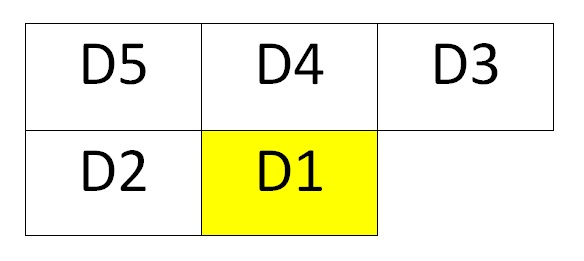
\includegraphics[width=\textwidth]{ind_sasiedztwo.jpg}
	\caption{Sąsiedztwo piksela brane pod uwagę przy indeksacji}
	\label{fig:ind_sasiedztwo}
\end{figure}
%TODO za duży rysunek

W~pierwszym przypadku pikselowi zostaje przypisana nowa etykieta. 
Gdy spełniony jest warunek $b$, punkt otrzymuje etykietę $L$, natomiast jeśli zachodzi przypadek $c$, przypisywana jest mniejsza z~etykiet. 
W~ten sposób otrzymuje się obraz wstępnie poetykietowany. 
Najczęściej posiada on więcej przypisanych etykiet, niż obiektów. 
Dlatego istnieje konieczność złączenia ze~sobą pewnych etykiet przy użyciu tablicy sklejeń. 
Tablica ta zawiera informację, które etykiety powinny zostać złączone. 
W~przypadku~$a$ do tablicy sklejeń na~pozycji odpowiadającej etykiecie zapisywana jest etykieta, natomiast gdy zachodzi opcja~$c$ etykietę mniejszą zapisuje się pod indeksem większej. 
Do sklejenia etykiet potrzebna jest druga iteracja, tym razem po~obrazie wstępnie poetykietowanym.\\

Powyższy fakt jest główną przeszkodą w~łatwym wykonaniu takiego algorytmu w~systemie potokowym. 
Bez~zapamiętywania całej ramki, w~przypadku sklejania etykiet, niemożliwy jest powrót do~wcześniej przetwarzanych pikseli. 
Pomimo tego, możliwe jest obliczenie pewnych cech obiektów, takich jak: pole, współrzędne środka ciężkości, prostokąt otaczający. 
W~pracy \cite{COG} podano sposób, w~jaki można tego dokonać. 
Opiera się on~na~scaleniu nie samych wartości pikseli, ale~obliczanych na~bieżąco parametrów obiektu.\\ 
Implementacja w~języku Verilog rodzi dodatkowo trudności związane z~określeniem przypadku istnienia tej~samej lub~różnych etykiet w~otoczeniu piksela. 
Utrudnienie stanowi brak możliwości wykorzystania funkcji eliminującej zera z~wektora, czy znajdującej minimum i~maksimum. %TODO niejasne
O~ile~wykrycie przypadku $a$ jest łatwe, to~przypadki $b$~i~$c$ wymagały rozważenia kilku możliwości. 
Zdecydowano się na~wykrywanie ich za~pomocą flag bitowych. 
Na~ich podstawie wnioskowano o~zachodzącym aktualnie przypadku oraz wskazywano, od~którego piksela z~otoczenia powinna zostać przepisana etykieta. 
Oprócz tego, na bieżąco obliczano prostokąt otaczający oraz liczbę pikseli należących do~każdego ze~znalezionych obiektów.\\
%TODO No a co z tworzeniem tablicy sklejeń ?

Po poetykietowaniu całej ramki obrazu wykorzystano tablicę sklejeń do~złączenia obliczanych na~bieżąco cech. 
Ten~etap algorytmu zaimplementowano jako maszynę stanów:
\begin{itemize}
	\item Stan 0 -- Oczekiwanie na sygnał końca ramki wyznaczany na podstawie synchronizacji pionowej. W~momencie wykrycia sygnału następuje rejestrowanie tablicy sklejeń i~obliczonych parametrów, zerowanie tablic wypełnianych w~kolejnym etapie oraz przejście do~stanu~1. %TODO rejestreowanie, czy resetowanie ?
	\item Stan 1 -- Iteracja po tablicy sklejeń i~uzupełnianie rzeczywistych wartości cech obiektów.
	\item Stan 2 -- Uporządkowanie tablic z~wyznaczonymi parametrami.
	\item Stan 3 -- Obliczenie pola prostokąta otaczającego dla każdego znalezionego obiektu. Wykorzystywana jest mnożarka o~latencji 3.
	\item Stan 4 -- Szukanie obiektu spełniającego warunki minimalnej wielkości pola powierzchni oraz stosunku pola prostokąta otaczającego do pola obiektu. W~przypadku znalezienia takiego kształtu, na~wyjście trafiają współrzędne jego prostokąta otaczającego. Jeśli żądany kształt nie zostanie znaleziony, informacja o~tym również pojawi się na~wyjściu.
\end{itemize}
Schemat przetwarzania danych po~każdej ramce pokazano na rysunku \ref{fig:ind_schemat}
\begin{figure}[h]
	\centering
	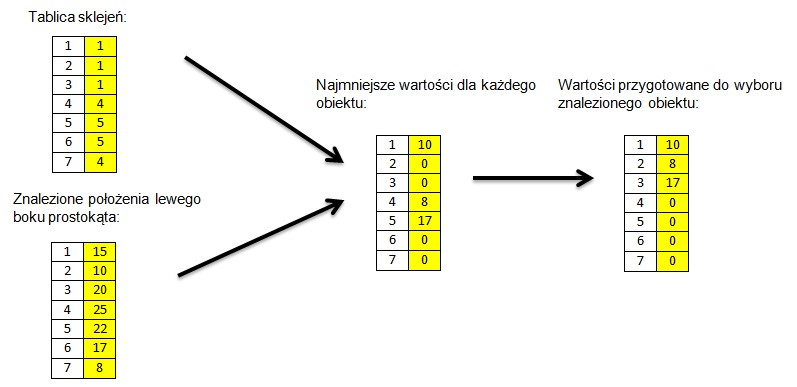
\includegraphics[width=\textwidth]{ind_schemat.jpg}
	\caption{Schemat procesu przetwarzania informacji po~każdej ramce obrazu z przykładowymi danymi.}
	\label{fig:ind_schemat}
\end{figure}
%TODO Schemat niejasny.

Główną trudnością w~implementacji opisanego algorytmu w~układzie FPGA jest stosunkowo duże zapotrzebowanie na~zasoby sprzętowe. 
Należy zarezerwować miejsce na~cechy każdego potencjalnego obiektu. 
Ogranicza to~liczbę możliwych etykiet. 
Zarezerwowanie miejsca dla 30~obiektów nie~przekroczyło możliwości układu Zybo. 
Badania pokazały, że~jest to wystarczająca liczba etykiet do~sprawnego działania toru wizyjnego.

%TODO 1. Zostało to zaimplementowane ?
%TODO 2. Skoro indeksacja to po co wcześniejszy środek ciężkości

\section{Komunikacja układu ZYBO Z7-20 ze sterownikiem Pixhawk}
\label{sec:komunikacja_ukladu_ZYBO_ze_sterownikiem_ Pixhawk} 
--- Tutaj chciałbym opisać protokół Mavlink używany do komunikacji ze sterownikiem. Obecnie została nawiązana komunikacja i udało się wysłać komendę uzbrojenia drona w trybie STABILIZE. W najbliższym czasie planuję przeprowadzić test wysyłania komend ruchu w trybie GUIDED, który wymaga połączenia GPS.
%-------------------------------------------------------------------------
